\section{Results}

The spatial and spectral averages are plotted against each other in figure 
\begin{figure}[h]
    \centering
    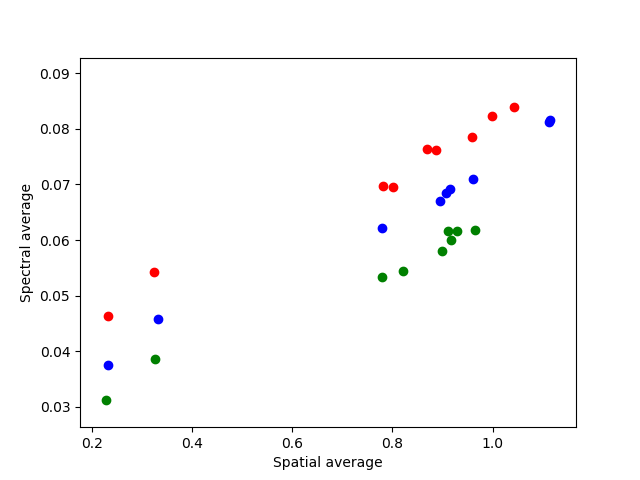
\includegraphics[width=1\textwidth]{Plots/spectral_vs_spatial_average.png}
    \caption{Spatial and spectral averages plotted against each other}
    \label{fig:spectral_vs_spatial_values}
\end{figure}



\section{Discussion}
The spatial and spectral averages should be codependent. This is because we have the same type of sensor, that are imaging the area in two different ways, but through taking the average to eliminate that difference it should amount to proportional values. 
